\documentclass[12pt]{article}

% Language setting
% Replace `english' with e.g. `spanish' to change the document language
\usepackage[english]{babel}
\usepackage[margin=1.2in]{geometry}
\usepackage{amsmath}
\usepackage{graphicx}
\usepackage[colorlinks=true, allcolors=blue]{hyperref}
\usepackage[skip=\medskipamount]{parskip}

\setlength\parindent{0pt}

\title{Variability in female Northern Cardinal calls: How do female songbirds sing? 
}
\author{MCB/Neuro 105\\Spring 2023\\Prof. Engert\\Jocelyn Hsieh}

\begin{document}
\maketitle

\begin{abstract}
    There is some sexual dimorphism among songbirds: most males sing songs to attract female mates, while it has long been believed that female songbirds do not sing. However, though there is evidence of singing in female songbirds, especially since song was likely a precursor to the sexual dimorphism observed now, not much research exists on the act of song in female songbirds \cite{Riebel}. Here, we seek to find the analogous systems that account for variability in female songbird songs. By identifying the similarities and differences with male songbirds, we may be better equipped to evaluate the reasons for songs in female birds and/or the reasons for the evolution of sexual dimorphisms in birdsong. 
\end{abstract}

\section{Introduction}
The song systems found in male songbirds are typically atrophied in females \cite{Mooney1}. There has been some research regarding the role of parts of the brain implicated in song-learning in female/juvenile birds, mainly on highly sexually-dimorphic zebra finches: experience plays a large role in female songbird learning, and songs heard in development play a role in mate preference, similar to how males use experience in development for the songs they sing later in life \cite{Fujii}. 

There are two main parts of the song system: the song motor pathway (SMP), implicated in the variability of actual songs in male songbirds, and the anterior forebrain pathway (AFP), which is heavily used in learning songs during development. A diagram is included in Figure \ref{fig:song_circuit}.

Previous research on female songbirds focuses on the AFP, which includes the thalamus and its immediate processing regions: Field L, as well as the medial caudal mesopallium (CMM), caudal nidopallium (NC), and the high vocal center (HVC). The CMM has been shown to behave similarly in males and females, and plays a role in mate preference and reward. The NC has been found to code for familiarity, coding social behaviors with familiar male birds \cite{Fujii}. The HVC in male songbirds appears to act as mirror neurons, firing both when the bird sings its song or hears its own song, but does not play a role in preference in female birds. 

In male songbirds, lesions to the output nucleus of the SMP (LMAN) result in reduced variability of songs \cite{Mooney1}. However, in non-singing female birds like the zebra finch, the size of the LMAN is much reduced \cite{Nixdorf}. 

\begin{figure}[ht]
\centering
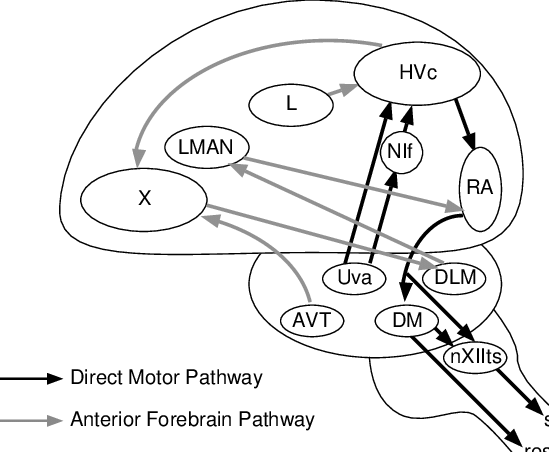
\includegraphics[width=0.5\textwidth]{song_circuit.png}
\caption{\label{fig:song_circuit}The song circuit found in male zebra finches.}
\end{figure}

We also define important terms in evaluating birdsong. Here, we will define a syllable for every vocalization that is separated by at least 5 ms from the next pitch. A motif is a run of syllables that is repeated, and a song or bout is a period of vocalization that contains at least one motif and is separated by the next vocalization by at least 500 ms.


\section{Aims}
    The goal of this study is to evaluate the differences between male and female songbirds, specifically by documenting the key elements in the song circuit for singing female songbirds. The study will use Northern Cardinals as a model organism, in contrast to the non-singing zebra finches that are traditionally used. We expect to find similar, albeit less crystallized, circuits in female songbirds as in male songbirds, such that the Cardinals may learn new songs with lower fidelity. Such a finding would challenge the assumption that the purpose of song in songbirds is to attract mates, as female Northern Cardinals choose their mates.


% \subsection{How to add Citations and a References List}

% You can simply upload a \verb|.bib| file containing your BibTeX entries, created with a tool such as JabRef. You can then cite entries from it, like this: \cite{greenwade93}. Just remember to specify a bibliography style, as well as the filename of the \verb|.bib|. You can find a \href{https://www.overleaf.com/help/97-how-to-include-a-bibliography-using-bibtex}{video tutorial here} to learn more about BibTeX.

% If you have an \href{https://www.overleaf.com/user/subscription/plans}{upgraded account}, you can also import your Mendeley or Zotero library directly as a \verb|.bib| file, via the upload menu in the file-tree.

\section{Methods}

We test three main functionalities in the song circuit: the LMAN in song variability, HVC$_{RA}$ neurons in tempo control, and HVC$_X$ neurons in mirroring activity.

\subsection{Evaluate the role of the LMAN in song variability in female Northern Cardinals by lesioning.}
We will create small lesions in female Northern Cardinals and compare the resulting songs for new and known songs: female Cardinals most commonly sing duets with male Cardinals during courtship, and often imitate male songs during this period. We will test the stereotypy in pitch and syllable duration pre- and post-lesioning.

First, we will record female birdsong in duet with their mates prior to lesioning for 5-10 Cardinals. Since the mating period for mating pairs can be predicted to begin in March and typically lasts for two months, we can reasonably allow the learning period for duet songs to continue for three weeks. Then, we will lesion the female Cardinal’s LMAN. To create lesions, we will induce bilateral electrolytic lesioning on the LMAN. We will then play back the male’s learned songs from the learning period and record the female bird’s songs. We will also play new songs from the same male, likely from past breeding seasons, and record the female bird’s response.

To distinguish measurements of frequency and syllable duration, we will first need to label distinct syllables prior to lesioning. We can transcribe the recordings, measured in Hz, into spectrograms. An example of such labeling is in Figure \ref{fig:spectrograph}. Trained observers will cluster similar syllables to the same labels; we can also train a neural network to automate this process.

\begin{figure}[ht]
\centering
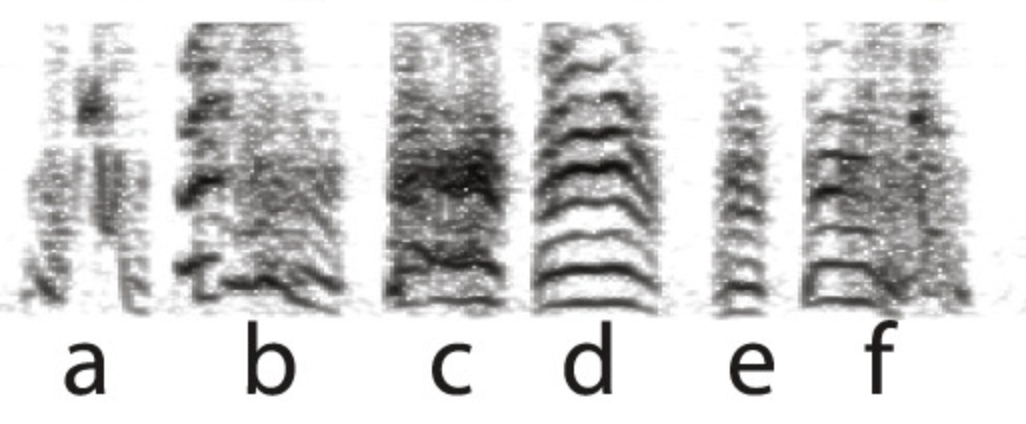
\includegraphics[width=0.7\textwidth]{sample_spectrograph.png}
\caption{\label{fig:spectrograph}A sample labeled spectrograph \cite{Moorman}.}
\end{figure}

We will measure pitch using the frequency recorded for each successive syllable recorded. We will measure syllable duration as the amount of time from the beginning of each syllable to its end. We will compare the coefficient of variation (CV = SD/mean) to pre-lesioning results for both of these measurements. Additionally, we will measure the naive rate of error in syllable sequence per bout/song: $\frac{\text{incorrect syllables}}{\text{total syllables}}$ \cite{Moorman}.

\subsection{Evaluate the role of the HVC$_{RA}$ in determining female Northern Cardinal song tempo by cooling the HVC.}

In male zebra finches, it has been observed that HVC$_{RA}$ neurons fire once per motif or during rests in the song, such that the ensemble of firing aligns with the tempo of the song. When cooled, the duration of motifs, syllables, and inter-syllable gaps were all elongated. However, the effect was more pronounced on the HVC$_{RA}$ transmission than on the song itself, indicating that the HVC is likely part of a distributed system that controls song tempo. No similar experiments have been conducted in singing female songbirds. As in previous studies, we will cool the HVC with a Peltier device (Figure \ref{fig:peltier}) and measure the resulting syllable duration changes  and firing rate change of HVC$_{RA}$ neurons in female Northern Cardinals. 

\begin{figure}[ht]
\centering
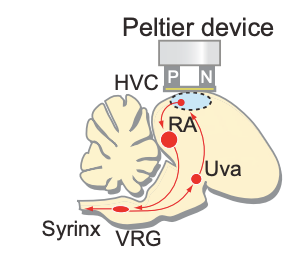
\includegraphics[width=0.3\textwidth]{hvc_peltier.png}
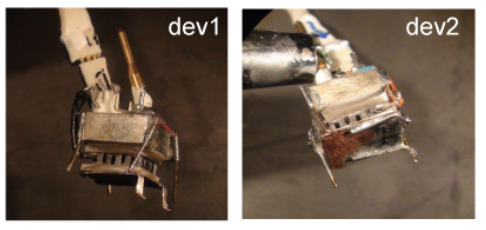
\includegraphics[width=0.5\textwidth]{irl_peltier.png}
\caption{\label{fig:peltier} A miniature Peltier device, as used to cool the HVC \cite{Hamaguchi}.}
\end{figure}

First, we will place a miniature Peltier device over the bird HVC for 5-10 female Cardinals. We cool the HVC from the original temperature of the brain, ($\sim 40^{o}C$). We will then take intracellular recordings of HVC$_{RA}$ neurons, before and during cooling. To calculate the latency of these neurons from cooling, we will align electrical stimulation, then measure the average delay between stimulation and synaptic firing.

We will additionally measure the syllable duration as described in the previous experiment, both prior to and during cooling. The duration is from the start of vocalization to the end, where syllables are separated by 5ms; we can reuse the labeling scheme from 3.1.

We then evaluate the effect of the cooling on the timing of the above measures and calculate the $Q_{10}$ values, or the change in timing per $10^o$C decrease in temperature. Specifically, let $T1, T2$ be the temperature in the brain before and during cooling, respectively, and let $L1, L2$ be the mean duration or latency for the respective temperatures. Then $$Q_{10} = (L1/L2)^{\frac{10}{T2-T1}}$$

To interpret this data, if the cooling has no effect on timing, we expect $Q_{10} = 1$, while $Q_{10} = 2$ indicates that timing slows by a factor of 2 when the temperature cools $10^o$ \cite{Hamaguchi}.

\subsection{Observe mirror HVC$_X$ neurons in female Northern Cardinals as a result of either singing, hearing its own song, or hearing a male songbird.}

Since HVC$_X$ neurons act as mirror neurons in male songbirds, we want to find if this holds true for singing female songbirds as well \cite{Mooney2}. Importantly, since female songbirds typically listen to songs to choose mates, we want to record the activity of such neurons both during female song, when it hears its own song, and while it’s listening to male songbirds: both familiar and unfamiliar. Similarly, as comparison, we will want to record the same recordings for male Cardinals.

We will record extracellular activity from neurons in the HVC by implanting thin microelectrodes into the region (microdrive). We can discriminate individual neurons by the amplitudes of action potentials and existence of refractory periods. We will then record activity from many neurons while the Northern Cardinal is:
\begin{enumerate}
    \item singing its own song, ideally in a solo and not a duet.
    \item listening to its own song.
    \item listening to its mate singing the same mating song.
    \item listening to an unrelated male Northern Cardinal.
\end{enumerate}

To analyze the data, we will align the beginnings of the songs and run paired student-$t$ tests to compare the means of neuronal activity \cite{Prather}.

\section{Expected Results}
Generally, we will expect the female Cardinals to express less stability or more variability in their learned songs (i.e. decreased stereotypy) compared to male Cardinals.

\subsection{LMAN role in pitch and syllable duration stability.}
Upon hearing a learned song, we expect for decreased variability in the female's pitch and syllable duration (lower CV value). The error rate should not change from prior to lesioning, given that the song is learned. However, the error rate may be higher than what is typically found in male Cardinals.

On hearing a new song, we expect either no response, or an unrelated song. Compared to an un-lesioned Cardinal learning a song, there will be significantly increased variability. In addition, there will be high rates of error.

\subsection{HVC$_{RA}$ role in song tempo}
Like in male songbirds, we expect increased $Q_{10}$ values for both syllable duration (a good marker for song slow-down) and HVC$_{RA}$ latency. In particular, we expect $Q_{10} \sim 1.3$ for syllable duration and $Q_{10} \sim 2$ for HVC$_{RA}$ latency \cite{Hamaguchi}. 

Since we also predict that stereotypy in female songbirds will be lower, we predict that the variance on latency and syllable duration data will be higher than in male songbirds; indeed, the $Q_{10}$ values may even be higher than predicted.

\subsection{HVC$_X$ neuronal responses in mirroring}
We expect the same mirroring activity in male and female Cardinals. Example activity in male swamp sparrows is included in Figure \ref{fig:hvc_results}. 

\begin{figure}[ht]
\centering
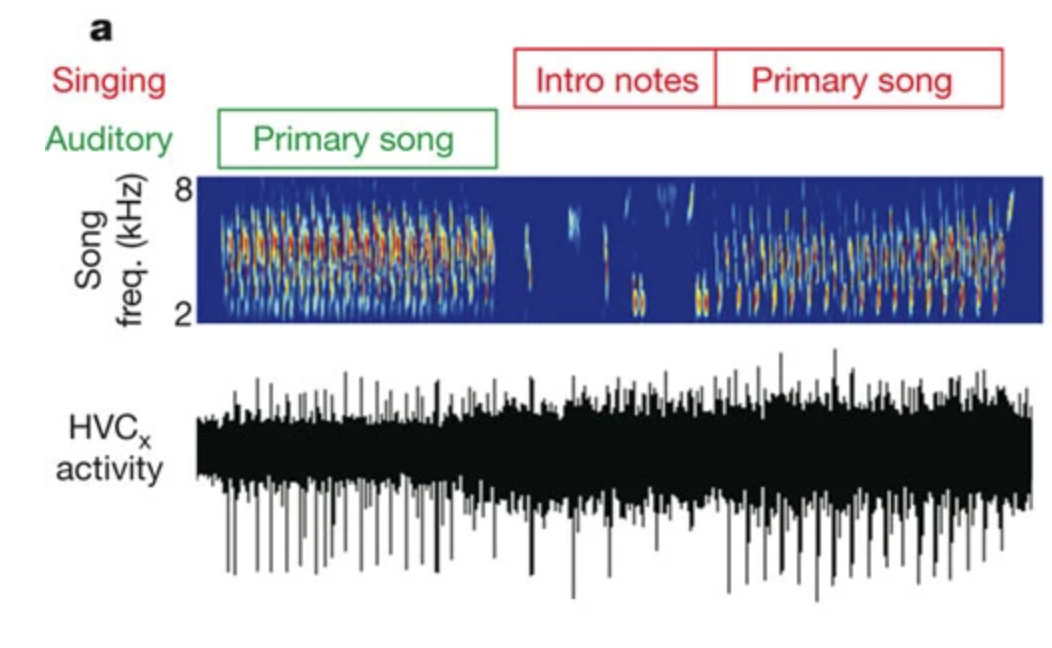
\includegraphics[width=0.7\textwidth]{hvc_results.png}
\caption{\label{fig:hvc_results}HVC$_X$ activity while listening to own song and while singing \cite{Prather}.}
\end{figure}

Further, similar to male Cardinals, we expect the same comparison of average activity (student-\textit{t} paired tests) across the first three tested conditions, but decreased HVC$_X$ activity when listening to unrelated males.

\section{Discussion}
From 4.1, we can interpret that the LMAN plays a similar role in both male and female songbirds \textit{given} that the female songbird in this instance, the Northern Cardinal, also displays song.

From 4.2, we further see that the HVC in female singing birds functions similar to in male songbirds, in that it can also inform the bird's control of the song. Furthermore, we can interpret the increased variance as evidence of sexual dimorphism, where the female evidently has less control over the song and thus introduces more variability even into its stereotyped songs.

From 4.3, we should note again that the HVC in singing female songbirds functions much like in male songbirds. That is, HVC$_X$ neurons fire not only on listening to familiar mates' songs, but even on its own songs and/or while it's singing.

These results may seem trivial, given that they corroborate known information about the song circuit. However, there is starkly little research on singing female songbirds, especially given that female song is relatively rare in songbirds. Therefore, it is probable that the results may differ from the expected ones; any such difference would provide much valuable information on the evolution of sexual dimorphism in the song circuit. Even with no new results, the main takeaway would reveal that there does exist a sexual dimorphism such that the main learning mechanisms are the same in female songbirds, but their ability to create the highly stereotyped songs is decreased. This is likely because female Cardinals don't need to sing to attract mates, so their ability to maintain difficult songs with high fidelity is less important.

Structures in the bird song circuit resemble regions in the human brain related to language learning and speech: the HVC is analogous to Broca's area in humans, and the LMAN functions  analogously to language learning in humans. Thus, any new understanding from the bird song circuit can inform our understanding of similar processes in humans. Furthermore, the major sexual dimorphism in songbirds is vastly different from the lack of dimorphism in humans; understanding how and why these differences emerged may help in our understanding of the species distinctions in brains. In other words, it may help to answer: at what point is a brain so different that it belongs to another species?

\section{Future Directions}
Preliminary research on structures in female singing songbirds is scarce, though some research on their recorded songs does exist. Therefore, much like research on human female bodies can be under-investigated, a more thorough understanding of the female song circuit is necessary to understand how and why such sexual dimorphism appeared. Furthermore, differences in female song circuits may offer a different perspective for the language circuit in human brains.

\newpage
\begin{thebibliography}{10}

\bibitem{Doya} Doya, K., \& Sejnowski, T. J. (1994, January 1). A novel reinforcement model of Birdsong Vocalization Learning: Proceedings of the 7th International Conference on Neural Information Processing Systems. Guide Proceedings. Retrieved April 25, 2023, from https://dl.acm.org/doi/10.5555/2998687.2998700 

\bibitem{Fujii} Fujii, Tomoko G., et al. Song Preference in Female and Juvenile Songbirds: Proximate and Ultimate Questions.\textit{ Frontiers in Physiology}, vol. 13, 2022, https://doi.org/10.3389/fphys.2022.876205.

\bibitem{Hamaguchi} Hamaguchi, K., Tanaka, M., \& Mooney, R. (2016). A distributed recurrent network contributes to temporally precise vocalizations. \textit{Neuron}, 91(3), 680–693. https://doi.org/10.1016/j.neuron.2016.06.019.

\bibitem{Mooney1} Mooney, R. (2014). Auditory–vocal mirroring in songbirds. \textit{Philosophical Transactions of the Royal Society B: Biological Sciences}, 369(1644), 20130179. https://doi.org/10.1098/rstb.2013.0179.

\bibitem{Mooney2} Mooney, R., et al. Neurophysiology of Birdsong Learning. \textit{Current Opinion in Neurobiology}, vol. 19, no. 6, Dec. 2009, pp. 654–660., https://doi.org/10.1016/b978-012370509-9.00116-9.

\bibitem{Moorman} Moorman, S., Ahn, J.-R., \& Kao, M. H. (2021). Plasticity of stereotyped birdsong driven by chronic manipulation of cortical-basal ganglia activity. \textit{Current Biology}, 31(12). https://doi.org/10.1016/j.cub.2021.04.030.

\bibitem{Nixdorf} Nixdorf-Bergweiler, Barbara E. Lateral Magnocellular Nucleus of the Anterior Neostriatum (LMAN) in the Zebra Finch: Neuronal Connectivity and the Emergence of Sex Differences in Cell Morphology. \textit{Microscopy Research and Technique,} vol. 54, no. 6, Sept. 2001, pp. 335–353., https://doi.org/10.1002/jemt.1147.

\bibitem{Prather} Prather, J. F., Peters, S., Nowicki, S., \& Mooney, R. (2008). Precise auditory–vocal mirroring in neurons for learned vocal communication. \textit{Nature}, 451(7176), 305–310. https://doi.org/10.1038/nature06492.

\bibitem{Riebel} Riebel, Katharina, et al. New Insights from Female Bird Song: Towards an Integrated Approach to Studying Male and Female Communication Roles. \textit{Biology Letters}, vol. 15, no. 4, 3 Apr. 2019, p. 20190059., https://doi.org/10.1098/rsbl.2019.0059.

\end{thebibliography}

\end{document}